\documentclass{article}
\usepackage{graphicx}
\usepackage{float}
\usepackage{amsmath}
\usepackage{amsfonts}
\usepackage{amssymb}
\usepackage{hyperref}
\usepackage{esint}
\usepackage[utf8]{inputenc}
\usepackage[a4paper, portrait, margin=0.75in]{geometry}
\setlength\parindent{0pt}
\usepackage[italian]{babel}
\usepackage{tikz}
\usepackage{circuitikz}





\hypersetup{
    colorlinks=true,
    linkcolor=black,
    filecolor=magenta,
    urlcolor=blue,
    pdftitle={Tecnologie internet},
    pdfpagemode=FullScreen,
}


\begin{document}
    \author{kanopo}
    \title{APPLICAZIONI INDUSTRIALI ELETTRICHE ED ELETTRONICA (MODULO 1)}
    \date{2022}

    \maketitle
    \tableofcontents

    \listoffigures
    \listoftables

    \section{Introduzione}

\subsection{Tensione}

L'unità di misura della tensione è il Volt $[V]$.


\begin{figure}[H]
    \centering
    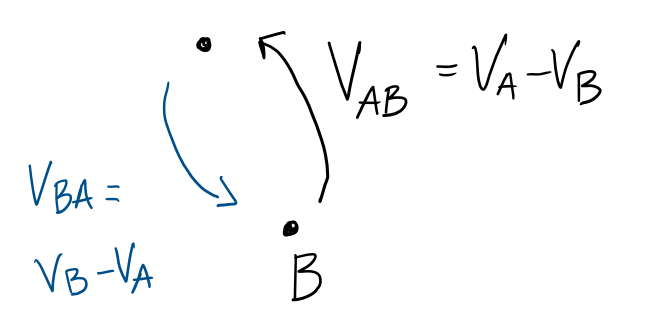
\includegraphics[width=0.3\linewidth]{1 - circuiti DC/imgs/Screenshot from 2022-06-09 17-14-50.png}
    \label{fig:tensione}
    \caption{Verso tensione}
\end{figure}

\subsection{Corrente}
L'unità di misura della corrente è il Ampere $[A]$.

\subsection{Legge di Ohm}
\subsubsection*{Prima legge}
La \textbf{resistenza} si indica con $R [\Omega]$(ohm) e si calcola:
\begin{equation*}
    V = R \cdot I
\end{equation*}


L'\textbf{induttanza} è l'opposto della resistenza e si indica con $G [S]$(Siemens)

\begin{equation*}
    R = \frac{1}{G}
\end{equation*}
\begin{equation*}
    I = G \cdot V
\end{equation*}

\subsubsection*{Seconda legge}

La \textbf{resistività} si indica con $\rho [\Omega \cdot m]$(ohm per metro) e si calcola:



L'\textbf{conducibilità} è l'opposto della resistività e si indica con $\sigma [\frac{S}{m}]$(Siemens fratto metri)
\begin{equation*}
    \rho = \frac{1}{\sigma}
\end{equation*}

\begin{equation*}
    R = \rho \cdot \frac{l}{S}
\end{equation*}

\begin{equation*}
    G = \sigma \cdot \frac{S}{l}
\end{equation*}
Dove $l$ è la lunghezza del materiale e $S$ è la sezione.

\subsection{Componenti reattivi}
\subsubsection{Condensatore}

\begin{equation*}
    Q = C \cdot V
\end{equation*}

\begin{equation*}
    \epsilon_C = \frac{1}{2} C\cdot V^2
\end{equation*}


In circuiti statici il condensatore viene visto come un pezzo di circuito aperto.

Quando siamo in presenza di una corrente variabile($i$) e di una tensione variabile($v$)(\textit{ovviamente}), usiamo queste formuline swag:

\begin{equation*}
    i = C \cdot \frac{\delta v}{\delta t}
\end{equation*}

\subsubsection{Induttore}

\begin{equation*}
    \lambda = L \cdot I
\end{equation*}

\begin{equation*}
    \epsilon_L = \frac{1}{2} L\cdot I^2
\end{equation*}

In circuiti statici il solenoide viene visto come un pezzo di circuito cortocircuitato.

Quando siamo in presenza di una corrente variabile($i$) e di una tensione variabile($v$)(\textit{ovviamente}), usiamo queste formuline swag:

\begin{equation*}
    i = L \cdot \frac{\delta i}{\delta t}
\end{equation*}

\subsection{Generatori dipendenti}
\begin{itemize}
    \item dipendenti da tensione
        \begin{itemize}
            \item Generatore di tensione dipendente da tensione (VCVS)
                \begin{equation*}
                    V = aV_x
                \end{equation*}
            \item Generatore di corrente dipendente da tensione (VCCS)
            \begin{equation*}
                I = bI_x
            \end{equation*}
        \end{itemize}
    \item dipendenti da corrente
        \begin{itemize}
            \item Generatore di tensione dipendente da corrente (CCVS)
                \begin{equation*}
                    V = rI_x
                \end{equation*}
            \item Generatore di corrente dipendente da corrente (CCCS)
                \begin{equation*}
                    I = gI_x
                \end{equation*}
        \end{itemize}
\end{itemize}

\subsection{Circuiti}

\begin{quotation}
    \textbf{Definizione}: Un \textbf{circuito} è un percorso chiuso che contiene componenti elettriche.
\end{quotation}

\begin{quotation}
    \textbf{Definizione}: Un \textbf{ramo} è una sequenza di componenti senza deviazioni?!
\end{quotation}
\begin{figure}[H]
    \centering
    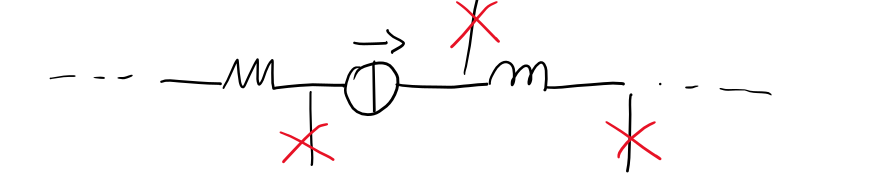
\includegraphics[width=0.5\linewidth]{1 - circuiti DC/imgs/Screenshot from 2022-06-09 22-43-00.png}
    \label{fig:rami}
    \caption{Esempio di ramo}
\end{figure}

\begin{quotation}
    \textbf{Definizione}: Un \textbf{nodo} è un punto d'incontro di 3 o più rami.
\end{quotation}

\begin{quotation}
    \textbf{Definizione}: Un \textbf{maglia} è percorso chiuso in un circuito
\end{quotation}
    \section{Metodo dei nodi}

\subsection{Leggi di Kirchhoff}
\subsubsection{Prima L.D.K delle correnti(KCL)}
\begin{quote}
    La somma algebrica delle correnti dei rami convergenti in un nodo è sempre nulla.
\end{quote}


\subsubsection{Seconda L.D.K delle tensioni(KVL)}
\begin{quote}
    La somma algebrica delle tensioni lungo una maglia è sempre nulla.
\end{quote}

\subsection{Metodo dei nodi}

\begin{enumerate}
    \item Identificare i nodi e fra questi decidere quale è il nodo di riferimento
    \item Identificare i versi (in modo arbitrario) delle correnti di ciascun ramo
    \item Scrivere le equazioni costitutive dei modelli dei componenti per esprimere le correnti di cui al punto 2 in funzione dei soli potenziali fra i nodi
        \begin{enumerate}
            \item se ancora vi sono correnti non in funzione dei potenziali, applicare KVL
        \end{enumerate}

    \item Risolvere il sistema che ha come incognite i soli potenziali di nodo
    \item Se necessario, determinare le altre tensioni con la KVL e le correnti usando le eqauzioni dei componenti
\end{enumerate}



    \section{Metodo agli anelli}

\subsection{Metodo degli anelli / maglie}

\begin{enumerate}
    \item Identificare gli anelli e attribuire loro un verso di percorrenza.
    \item identificare i versi delle tensioni di ciascun componente ad anello
    \item scrivere la KVL per tutti gli anelli
    \item Utilizzare le equazioni costitutive per esprimere le tensioni di cui al punto 2 in funzione dele solo correnti di maglia.
        \begin{enumerate}
            \item se ci sono ancora formule non in funzione della corrente, applicare KCL
        \end{enumerate}
    \item risolvere il sistema che ha come incognite le correnti di maglia
    \item se serve, determinare le altre correnti con la KCL e le tensioni usando le equazioni costitutive.
\end{enumerate}








    
\end{document}